% Options for packages loaded elsewhere
\PassOptionsToPackage{unicode}{hyperref}
\PassOptionsToPackage{hyphens}{url}
%
\documentclass[
  doc]{apa6}
\usepackage{amsmath,amssymb}
\usepackage{iftex}
\ifPDFTeX
  \usepackage[T1]{fontenc}
  \usepackage[utf8]{inputenc}
  \usepackage{textcomp} % provide euro and other symbols
\else % if luatex or xetex
  \usepackage{unicode-math} % this also loads fontspec
  \defaultfontfeatures{Scale=MatchLowercase}
  \defaultfontfeatures[\rmfamily]{Ligatures=TeX,Scale=1}
\fi
\usepackage{lmodern}
\ifPDFTeX\else
  % xetex/luatex font selection
\fi
% Use upquote if available, for straight quotes in verbatim environments
\IfFileExists{upquote.sty}{\usepackage{upquote}}{}
\IfFileExists{microtype.sty}{% use microtype if available
  \usepackage[]{microtype}
  \UseMicrotypeSet[protrusion]{basicmath} % disable protrusion for tt fonts
}{}
\makeatletter
\@ifundefined{KOMAClassName}{% if non-KOMA class
  \IfFileExists{parskip.sty}{%
    \usepackage{parskip}
  }{% else
    \setlength{\parindent}{0pt}
    \setlength{\parskip}{6pt plus 2pt minus 1pt}}
}{% if KOMA class
  \KOMAoptions{parskip=half}}
\makeatother
\usepackage{xcolor}
\usepackage{color}
\usepackage{fancyvrb}
\newcommand{\VerbBar}{|}
\newcommand{\VERB}{\Verb[commandchars=\\\{\}]}
\DefineVerbatimEnvironment{Highlighting}{Verbatim}{commandchars=\\\{\}}
% Add ',fontsize=\small' for more characters per line
\usepackage{framed}
\definecolor{shadecolor}{RGB}{248,248,248}
\newenvironment{Shaded}{\begin{snugshade}}{\end{snugshade}}
\newcommand{\AlertTok}[1]{\textcolor[rgb]{0.94,0.16,0.16}{#1}}
\newcommand{\AnnotationTok}[1]{\textcolor[rgb]{0.56,0.35,0.01}{\textbf{\textit{#1}}}}
\newcommand{\AttributeTok}[1]{\textcolor[rgb]{0.13,0.29,0.53}{#1}}
\newcommand{\BaseNTok}[1]{\textcolor[rgb]{0.00,0.00,0.81}{#1}}
\newcommand{\BuiltInTok}[1]{#1}
\newcommand{\CharTok}[1]{\textcolor[rgb]{0.31,0.60,0.02}{#1}}
\newcommand{\CommentTok}[1]{\textcolor[rgb]{0.56,0.35,0.01}{\textit{#1}}}
\newcommand{\CommentVarTok}[1]{\textcolor[rgb]{0.56,0.35,0.01}{\textbf{\textit{#1}}}}
\newcommand{\ConstantTok}[1]{\textcolor[rgb]{0.56,0.35,0.01}{#1}}
\newcommand{\ControlFlowTok}[1]{\textcolor[rgb]{0.13,0.29,0.53}{\textbf{#1}}}
\newcommand{\DataTypeTok}[1]{\textcolor[rgb]{0.13,0.29,0.53}{#1}}
\newcommand{\DecValTok}[1]{\textcolor[rgb]{0.00,0.00,0.81}{#1}}
\newcommand{\DocumentationTok}[1]{\textcolor[rgb]{0.56,0.35,0.01}{\textbf{\textit{#1}}}}
\newcommand{\ErrorTok}[1]{\textcolor[rgb]{0.64,0.00,0.00}{\textbf{#1}}}
\newcommand{\ExtensionTok}[1]{#1}
\newcommand{\FloatTok}[1]{\textcolor[rgb]{0.00,0.00,0.81}{#1}}
\newcommand{\FunctionTok}[1]{\textcolor[rgb]{0.13,0.29,0.53}{\textbf{#1}}}
\newcommand{\ImportTok}[1]{#1}
\newcommand{\InformationTok}[1]{\textcolor[rgb]{0.56,0.35,0.01}{\textbf{\textit{#1}}}}
\newcommand{\KeywordTok}[1]{\textcolor[rgb]{0.13,0.29,0.53}{\textbf{#1}}}
\newcommand{\NormalTok}[1]{#1}
\newcommand{\OperatorTok}[1]{\textcolor[rgb]{0.81,0.36,0.00}{\textbf{#1}}}
\newcommand{\OtherTok}[1]{\textcolor[rgb]{0.56,0.35,0.01}{#1}}
\newcommand{\PreprocessorTok}[1]{\textcolor[rgb]{0.56,0.35,0.01}{\textit{#1}}}
\newcommand{\RegionMarkerTok}[1]{#1}
\newcommand{\SpecialCharTok}[1]{\textcolor[rgb]{0.81,0.36,0.00}{\textbf{#1}}}
\newcommand{\SpecialStringTok}[1]{\textcolor[rgb]{0.31,0.60,0.02}{#1}}
\newcommand{\StringTok}[1]{\textcolor[rgb]{0.31,0.60,0.02}{#1}}
\newcommand{\VariableTok}[1]{\textcolor[rgb]{0.00,0.00,0.00}{#1}}
\newcommand{\VerbatimStringTok}[1]{\textcolor[rgb]{0.31,0.60,0.02}{#1}}
\newcommand{\WarningTok}[1]{\textcolor[rgb]{0.56,0.35,0.01}{\textbf{\textit{#1}}}}
\usepackage{graphicx}
\makeatletter
\def\maxwidth{\ifdim\Gin@nat@width>\linewidth\linewidth\else\Gin@nat@width\fi}
\def\maxheight{\ifdim\Gin@nat@height>\textheight\textheight\else\Gin@nat@height\fi}
\makeatother
% Scale images if necessary, so that they will not overflow the page
% margins by default, and it is still possible to overwrite the defaults
% using explicit options in \includegraphics[width, height, ...]{}
\setkeys{Gin}{width=\maxwidth,height=\maxheight,keepaspectratio}
% Set default figure placement to htbp
\makeatletter
\def\fps@figure{htbp}
\makeatother
\setlength{\emergencystretch}{3em} % prevent overfull lines
\providecommand{\tightlist}{%
  \setlength{\itemsep}{0pt}\setlength{\parskip}{0pt}}
\setcounter{secnumdepth}{-\maxdimen} % remove section numbering
% Make \paragraph and \subparagraph free-standing
\makeatletter
\ifx\paragraph\undefined\else
  \let\oldparagraph\paragraph
  \renewcommand{\paragraph}{
    \@ifstar
      \xxxParagraphStar
      \xxxParagraphNoStar
  }
  \newcommand{\xxxParagraphStar}[1]{\oldparagraph*{#1}\mbox{}}
  \newcommand{\xxxParagraphNoStar}[1]{\oldparagraph{#1}\mbox{}}
\fi
\ifx\subparagraph\undefined\else
  \let\oldsubparagraph\subparagraph
  \renewcommand{\subparagraph}{
    \@ifstar
      \xxxSubParagraphStar
      \xxxSubParagraphNoStar
  }
  \newcommand{\xxxSubParagraphStar}[1]{\oldsubparagraph*{#1}\mbox{}}
  \newcommand{\xxxSubParagraphNoStar}[1]{\oldsubparagraph{#1}\mbox{}}
\fi
\makeatother
% definitions for citeproc citations
\NewDocumentCommand\citeproctext{}{}
\NewDocumentCommand\citeproc{mm}{%
  \begingroup\def\citeproctext{#2}\cite{#1}\endgroup}
\makeatletter
 % allow citations to break across lines
 \let\@cite@ofmt\@firstofone
 % avoid brackets around text for \cite:
 \def\@biblabel#1{}
 \def\@cite#1#2{{#1\if@tempswa , #2\fi}}
\makeatother
\newlength{\cslhangindent}
\setlength{\cslhangindent}{1.5em}
\newlength{\csllabelwidth}
\setlength{\csllabelwidth}{3em}
\newenvironment{CSLReferences}[2] % #1 hanging-indent, #2 entry-spacing
 {\begin{list}{}{%
  \setlength{\itemindent}{0pt}
  \setlength{\leftmargin}{0pt}
  \setlength{\parsep}{0pt}
  % turn on hanging indent if param 1 is 1
  \ifodd #1
   \setlength{\leftmargin}{\cslhangindent}
   \setlength{\itemindent}{-1\cslhangindent}
  \fi
  % set entry spacing
  \setlength{\itemsep}{#2\baselineskip}}}
 {\end{list}}
\usepackage{calc}
\newcommand{\CSLBlock}[1]{\hfill\break\parbox[t]{\linewidth}{\strut\ignorespaces#1\strut}}
\newcommand{\CSLLeftMargin}[1]{\parbox[t]{\csllabelwidth}{\strut#1\strut}}
\newcommand{\CSLRightInline}[1]{\parbox[t]{\linewidth - \csllabelwidth}{\strut#1\strut}}
\newcommand{\CSLIndent}[1]{\hspace{\cslhangindent}#1}
\ifLuaTeX
\usepackage[bidi=basic]{babel}
\else
\usepackage[bidi=default]{babel}
\fi
\babelprovide[main,import]{english}
% get rid of language-specific shorthands (see #6817):
\let\LanguageShortHands\languageshorthands
\def\languageshorthands#1{}
% Manuscript styling
\usepackage{upgreek}
\captionsetup{font=singlespacing,justification=justified}

% Table formatting
\usepackage{longtable}
\usepackage{lscape}
% \usepackage[counterclockwise]{rotating}   % Landscape page setup for large tables
\usepackage{multirow}		% Table styling
\usepackage{tabularx}		% Control Column width
\usepackage[flushleft]{threeparttable}	% Allows for three part tables with a specified notes section
\usepackage{threeparttablex}            % Lets threeparttable work with longtable

% Create new environments so endfloat can handle them
% \newenvironment{ltable}
%   {\begin{landscape}\centering\begin{threeparttable}}
%   {\end{threeparttable}\end{landscape}}
\newenvironment{lltable}{\begin{landscape}\centering\begin{ThreePartTable}}{\end{ThreePartTable}\end{landscape}}

% Enables adjusting longtable caption width to table width
% Solution found at http://golatex.de/longtable-mit-caption-so-breit-wie-die-tabelle-t15767.html
\makeatletter
\newcommand\LastLTentrywidth{1em}
\newlength\longtablewidth
\setlength{\longtablewidth}{1in}
\newcommand{\getlongtablewidth}{\begingroup \ifcsname LT@\roman{LT@tables}\endcsname \global\longtablewidth=0pt \renewcommand{\LT@entry}[2]{\global\advance\longtablewidth by ##2\relax\gdef\LastLTentrywidth{##2}}\@nameuse{LT@\roman{LT@tables}} \fi \endgroup}

% \setlength{\parindent}{0.5in}
% \setlength{\parskip}{0pt plus 0pt minus 0pt}

% Overwrite redefinition of paragraph and subparagraph by the default LaTeX template
% See https://github.com/crsh/papaja/issues/292
\makeatletter
\renewcommand{\paragraph}{\@startsection{paragraph}{4}{\parindent}%
  {0\baselineskip \@plus 0.2ex \@minus 0.2ex}%
  {-1em}%
  {\normalfont\normalsize\bfseries\itshape\typesectitle}}

\renewcommand{\subparagraph}[1]{\@startsection{subparagraph}{5}{1em}%
  {0\baselineskip \@plus 0.2ex \@minus 0.2ex}%
  {-\z@\relax}%
  {\normalfont\normalsize\itshape\hspace{\parindent}{#1}\textit{\addperi}}{\relax}}
\makeatother

\makeatletter
\usepackage{etoolbox}
\patchcmd{\maketitle}
  {\section{\normalfont\normalsize\abstractname}}
  {\section*{\normalfont\normalsize\abstractname}}
  {}{\typeout{Failed to patch abstract.}}
\patchcmd{\maketitle}
  {\section{\protect\normalfont{\@title}}}
  {\section*{\protect\normalfont{\@title}}}
  {}{\typeout{Failed to patch title.}}
\makeatother

\usepackage{xpatch}
\makeatletter
\xapptocmd\appendix
  {\xapptocmd\section
    {\addcontentsline{toc}{section}{\appendixname\ifoneappendix\else~\theappendix\fi: #1}}
    {}{\InnerPatchFailed}%
  }
{}{\PatchFailed}
\makeatother
\keywords{counterfactual reasoning, Piaget, conservation theory, reversibility, cognitive development}
\usepackage{csquotes}
\usepackage{amsmath}
\ifLuaTeX
  \usepackage{selnolig}  % disable illegal ligatures
\fi
\usepackage{bookmark}
\IfFileExists{xurl.sty}{\usepackage{xurl}}{} % add URL line breaks if available
\urlstyle{same}
\hypersetup{
  pdftitle={PSY503 Final Project},
  pdfauthor={Bella Fascendini1},
  pdflang={en-EN},
  pdfkeywords={counterfactual reasoning, Piaget, conservation theory, reversibility, cognitive development},
  hidelinks,
  pdfcreator={LaTeX via pandoc}}

\title{PSY503 Final Project}
\author{Bella Fascendini\textsuperscript{1}}
\date{}


\shorttitle{Fascendini Final Project}

\authornote{

Department of Psychology, Princeton University

The authors made the following contributions. Bella Fascendini: Conceptualization, Data curation, Data analysis, Writing - Original Draft Preparation, Writing - Review \& Editing.

Correspondence concerning this article should be addressed to Bella Fascendini, Princeton University. E-mail: \href{mailto:bfascendini@princeton.edu}{\nolinkurl{bfascendini@princeton.edu}}

}

\affiliation{\phantom{0}}

\abstract{%
Conservation experiments are at the heart of Piaget's theory that young children are easily misled by appearances and fail to grasp that quantities are unaffected by superficial transformations. An independent line of research on the development of counterfactual thinking suggests that children struggle to imagine what the world would be if particular events had not occurred. Although seemingly unrelated, we suspect that counterfactual thinking might be in play when children perform mentally reversing changes in conservation tasks. The experiment reported here examines whether children's counterfactual thinking predicts their performance in solving conservation problems. Children (N = 48; 24 females) between 6 and 8 years old (72 - 95 months), completed conservation and counterfactual thinking tasks in a single Zoom session. In the conservation task, children received four conservation problems (liquid, mass, number, and length) delivered via pre-recorded video clips in which the experimenter altered the appearance of two qualitatively identical objects (e.g., a ball of modeling clay was reshaped to a flat sheet). In the counterfactual thinking task, children received four cartoon vignettes in which the experimenter described events live along with animated slides. In a given vignette, two simultaneous yet independent events caused the same outcome (e.g., a towel getting wet). Results showed that children's performance on the counterfactual thinking task significantly predicted their performance on the conservation task. Age also significantly predicted children's performance on both tasks. The findings suggest that there is a so-far undetected involvement of counterfactual thinking in solving conservation problems. We discuss the role of mentally reversing or undoing events in understanding the conservation of substance.
}



\begin{document}
\maketitle

\begin{Shaded}
\begin{Highlighting}[]
\CommentTok{\# Seed for random number generation}
\NormalTok{knitr}\SpecialCharTok{::}\NormalTok{opts\_chunk}\SpecialCharTok{$}\FunctionTok{set}\NormalTok{(}\AttributeTok{cache.extra =}\NormalTok{ knitr}\SpecialCharTok{::}\NormalTok{rand\_seed)}
\end{Highlighting}
\end{Shaded}

\section{Part 1 Reproducible report}\label{part-1-reproducible-report}

\subsection{Research question}\label{research-question}

This analysis examines how age and counterfactual thinking ability influence children's performance on conservation tasks. The study investigated whether children's understanding of conservation principles is related to their ability to reason counterfactually, and how this relationship might change with age.

\subsection{Data and Code for Re-analysis}\label{data-and-code-for-re-analysis}

\begin{Shaded}
\begin{Highlighting}[]
\FunctionTok{library}\NormalTok{(tidyverse)}
\FunctionTok{library}\NormalTok{(MetBrewer)}
\FunctionTok{library}\NormalTok{(lme4)}
\FunctionTok{library}\NormalTok{(nlme)}
\FunctionTok{library}\NormalTok{(scales)}
\CommentTok{\#set default theme for plots}
\FunctionTok{theme\_set}\NormalTok{(}\FunctionTok{theme\_classic}\NormalTok{() }\SpecialCharTok{+} 
            \FunctionTok{theme}\NormalTok{(}\AttributeTok{text =} \FunctionTok{element\_text}\NormalTok{(}\AttributeTok{size =} \DecValTok{12}\NormalTok{))) }
\end{Highlighting}
\end{Shaded}

\begin{Shaded}
\begin{Highlighting}[]
\NormalTok{data\_trialwise }\OtherTok{\textless{}{-}} \FunctionTok{read.csv}\NormalTok{(}\StringTok{"../data/data\_trialwise.csv"}\NormalTok{)}
\NormalTok{data\_summary }\OtherTok{\textless{}{-}} \FunctionTok{read.csv}\NormalTok{(}\StringTok{"../data/data\_summary.csv"}\NormalTok{)}

\FunctionTok{str}\NormalTok{(data\_trialwise)}
\FunctionTok{str}\NormalTok{(data\_summary)}
\end{Highlighting}
\end{Shaded}

\begin{Shaded}
\begin{Highlighting}[]
\CommentTok{\#Running logistic regression model, with performance on the counterfactual }
\CommentTok{\#reasoning task as a predictor of performance on conservation task}

\NormalTok{main\_model }\OtherTok{\textless{}{-}} \FunctionTok{glmer}\NormalTok{(post.transformation.score }\SpecialCharTok{\textasciitilde{}}\NormalTok{ Counterfactual\_total }\SpecialCharTok{+} 
\NormalTok{                      (}\DecValTok{1}\SpecialCharTok{|}\NormalTok{Subject), }\AttributeTok{family =} \FunctionTok{binomial}\NormalTok{(}\AttributeTok{link =} \StringTok{"logit"}\NormalTok{), }
                    \AttributeTok{data =}\NormalTok{ data\_trialwise)}

\FunctionTok{summary}\NormalTok{(main\_model)}
\end{Highlighting}
\end{Shaded}

\begin{Shaded}
\begin{Highlighting}[]
\CommentTok{\#Running logistic regression model, with age as the sole predictor of }
\CommentTok{\#performance on conservation task}
\NormalTok{age\_conservation\_model }\OtherTok{\textless{}{-}} \FunctionTok{glmer}\NormalTok{(post.transformation.score }\SpecialCharTok{\textasciitilde{}}\NormalTok{ Age.in.days }\SpecialCharTok{+} 
\NormalTok{                                  (}\DecValTok{1}\SpecialCharTok{|}\NormalTok{Subject),}
                \AttributeTok{family =} \FunctionTok{binomial}\NormalTok{(}\AttributeTok{link =} \StringTok{"logit"}\NormalTok{),}
                \AttributeTok{data =}\NormalTok{ data\_trialwise)}
\FunctionTok{summary}\NormalTok{(age\_conservation\_model)}
\end{Highlighting}
\end{Shaded}

\begin{Shaded}
\begin{Highlighting}[]
\CommentTok{\#Locating the source of the age effect in conservation }
\CommentTok{\#(could it have come from \#counterfactual \#reasoning? }
\CommentTok{\#This model includes age as the sole predictor of performance on the }
\CommentTok{\#counterfactual reasoning task)}

\NormalTok{age\_counterfactual\_model }\OtherTok{\textless{}{-}} \FunctionTok{glmer}\NormalTok{(Counterfactual\_score }\SpecialCharTok{\textasciitilde{}}\NormalTok{ Age.in.days }\SpecialCharTok{+} 
\NormalTok{                                    (}\DecValTok{1}\SpecialCharTok{|}\NormalTok{Subject),}
                \AttributeTok{family =} \FunctionTok{binomial}\NormalTok{(}\AttributeTok{link =} \StringTok{"logit"}\NormalTok{),}
                \AttributeTok{data =}\NormalTok{ data\_trialwise)}
\FunctionTok{summary}\NormalTok{(age\_counterfactual\_model)}
\end{Highlighting}
\end{Shaded}

\begin{Shaded}
\begin{Highlighting}[]
\CommentTok{\# This model includes both age and performance on the counterfactual reasoning }
\CommentTok{\#task as predictors of performance on the conservation task}

\NormalTok{age\_counterfactual\_conservation\_model}\OtherTok{\textless{}{-}} \FunctionTok{glmer}\NormalTok{(post.transformation.score }\SpecialCharTok{\textasciitilde{}} 
\NormalTok{                                                Age.in.days }\SpecialCharTok{+} 
\NormalTok{                                                Counterfactual\_total }\SpecialCharTok{+}
\NormalTok{                  (}\DecValTok{1}\SpecialCharTok{|}\NormalTok{Subject), }
                  \AttributeTok{family =} \FunctionTok{binomial}\NormalTok{(}\AttributeTok{link =} \StringTok{"logit"}\NormalTok{),}
                \AttributeTok{data =}\NormalTok{ data\_trialwise)}
\FunctionTok{summary}\NormalTok{(age\_counterfactual\_conservation\_model)}
\end{Highlighting}
\end{Shaded}

\begin{Shaded}
\begin{Highlighting}[]
\CommentTok{\# This model includes all demographic variables as predictors of }
\CommentTok{\#performance on the conservation task}

\NormalTok{demographic\_model }\OtherTok{\textless{}{-}} \FunctionTok{glmer}\NormalTok{(post.transformation.score }\SpecialCharTok{\textasciitilde{}}\NormalTok{ Gender }\SpecialCharTok{+}\NormalTok{ Age.in.days }\SpecialCharTok{+}
\NormalTok{                   Ethnicity }\SpecialCharTok{+}\NormalTok{ trial }\SpecialCharTok{+}\NormalTok{ Task\_order }\SpecialCharTok{+}
\NormalTok{                 Conservation\_Story }\SpecialCharTok{+}\NormalTok{ Conservation.question.order }\SpecialCharTok{+} 
\NormalTok{                   (}\DecValTok{1}\SpecialCharTok{|}\NormalTok{Subject),}
                 \AttributeTok{family =} \FunctionTok{binomial}\NormalTok{(}\AttributeTok{link =} \StringTok{"logit"}\NormalTok{), }
                 \AttributeTok{data =}\NormalTok{ data\_trialwise)}
\FunctionTok{summary}\NormalTok{(demographic\_model)}
\end{Highlighting}
\end{Shaded}

\begin{Shaded}
\begin{Highlighting}[]
\CommentTok{\#model comparison}
\FunctionTok{library}\NormalTok{(MuMIn)}
\FunctionTok{library}\NormalTok{(pROC)}

\CommentTok{\# Calculate AIC and BIC}
\FunctionTok{AIC}\NormalTok{(main\_model)}
\FunctionTok{AIC}\NormalTok{(age\_conservation\_model)}
\CommentTok{\# Repeat for other models}

\CommentTok{\# Calculate Pseudo{-}R\^{}2}
\FunctionTok{r.squaredGLMM}\NormalTok{(main\_model)}
\FunctionTok{r.squaredGLMM}\NormalTok{(age\_conservation\_model) }
\CommentTok{\# Repeat for other models}

\CommentTok{\# Predicted Probabilities and ROC Curve}
\NormalTok{main\_model\_probs }\OtherTok{\textless{}{-}} \FunctionTok{predict}\NormalTok{(main\_model, }\AttributeTok{type =} \StringTok{"response"}\NormalTok{)}
\NormalTok{age\_conservation\_probs }\OtherTok{\textless{}{-}} \FunctionTok{predict}\NormalTok{(age\_conservation\_model, }\AttributeTok{type =} \StringTok{"response"}\NormalTok{)}
\CommentTok{\# Repeat for other models}

\NormalTok{main\_model\_roc }\OtherTok{\textless{}{-}} \FunctionTok{roc}\NormalTok{(data\_trialwise}\SpecialCharTok{$}\NormalTok{post.transformation.score, }
\NormalTok{                      main\_model\_probs)}
\NormalTok{age\_conservation\_roc }\OtherTok{\textless{}{-}} \FunctionTok{roc}\NormalTok{(data\_trialwise}\SpecialCharTok{$}\NormalTok{post.transformation.score, }
\NormalTok{                            age\_conservation\_probs)}
\CommentTok{\# Repeat for other models and compare AUC values}

\CommentTok{\# Coefficient Comparison}
\FunctionTok{summary}\NormalTok{(main\_model)}
\FunctionTok{summary}\NormalTok{(age\_conservation\_model)}
\end{Highlighting}
\end{Shaded}

\begin{Shaded}
\begin{Highlighting}[]
\CommentTok{\# visualizing the distribution of children\textquotesingle{}s performance on both tasks. }

\FunctionTok{ggplot}\NormalTok{(data\_summary, }\FunctionTok{aes}\NormalTok{(}\AttributeTok{x =}\NormalTok{ counterfactual\_total, }\AttributeTok{y =}\NormalTok{ conservation\_total)) }\SpecialCharTok{+}
  \FunctionTok{geom\_count}\NormalTok{(}\FunctionTok{aes}\NormalTok{(}\AttributeTok{color =} \FunctionTok{after\_stat}\NormalTok{(n), }\AttributeTok{size =} \FunctionTok{after\_stat}\NormalTok{(n))) }\SpecialCharTok{+}
  \FunctionTok{guides}\NormalTok{(}\AttributeTok{color =} \StringTok{\textquotesingle{}legend\textquotesingle{}}\NormalTok{) }\SpecialCharTok{+}
  \CommentTok{\#scale\_size\_continuous(range = c(3, 7),breaks = 1:6) +}
  \FunctionTok{geom\_smooth}\NormalTok{(}\AttributeTok{method =}\NormalTok{ lm, }\AttributeTok{color =} \StringTok{"black"}\NormalTok{)}\SpecialCharTok{+}
  \FunctionTok{xlab}\NormalTok{(}\StringTok{"Counterfactual Task Score"}\NormalTok{) }\SpecialCharTok{+}
  \FunctionTok{ylab}\NormalTok{(}\StringTok{"Conservation Task Score"}\NormalTok{) }\SpecialCharTok{+}
  \FunctionTok{theme}\NormalTok{(}\AttributeTok{panel.background =} \FunctionTok{element\_blank}\NormalTok{()) }\SpecialCharTok{+} 
  \FunctionTok{theme}\NormalTok{(}\AttributeTok{axis.title.x =} \FunctionTok{element\_text}\NormalTok{(}\AttributeTok{size=}\DecValTok{14}\NormalTok{, }\AttributeTok{face=}\StringTok{"bold"}\NormalTok{),}
        \AttributeTok{axis.title.y =} \FunctionTok{element\_text}\NormalTok{(}\AttributeTok{size=}\DecValTok{14}\NormalTok{, }\AttributeTok{face=}\StringTok{"bold"}\NormalTok{),}
        \AttributeTok{axis.line =} \FunctionTok{element\_line}\NormalTok{(}\AttributeTok{colour =} \StringTok{"black"}\NormalTok{),}
        \AttributeTok{text =} \FunctionTok{element\_text}\NormalTok{(}\AttributeTok{size =} \DecValTok{12}\NormalTok{,}\AttributeTok{family=}\StringTok{"sans"}\NormalTok{), }
        \AttributeTok{axis.text.x =} \FunctionTok{element\_text}\NormalTok{(}\AttributeTok{colour=}\StringTok{"black"}\NormalTok{, }\AttributeTok{size =} \DecValTok{12}\NormalTok{,}\AttributeTok{family=}\StringTok{"sans"}\NormalTok{))}
\end{Highlighting}
\end{Shaded}

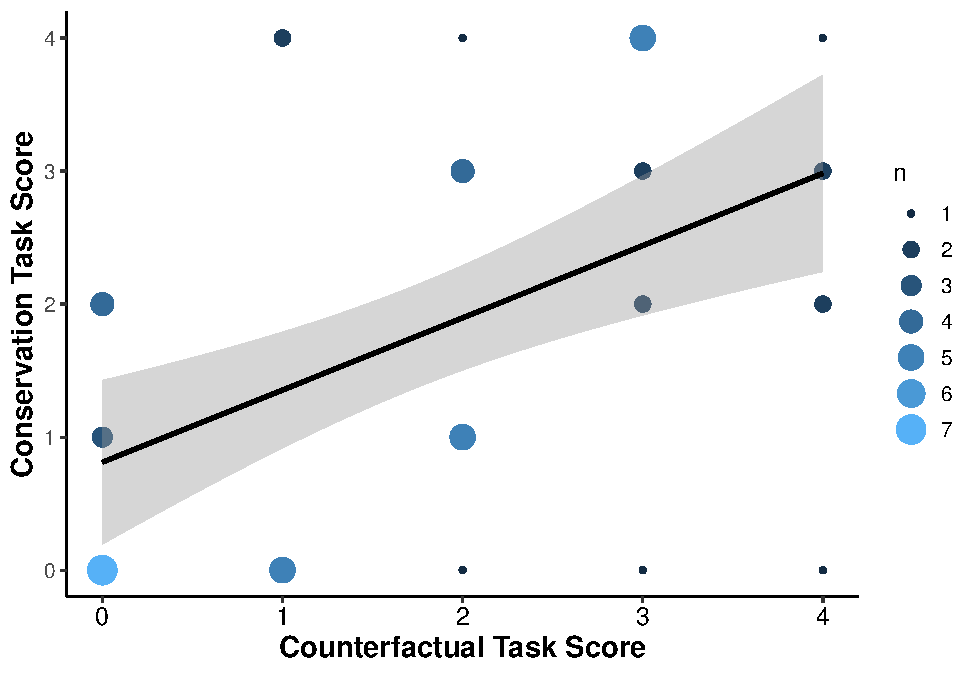
\includegraphics{final_project_files/figure-latex/unnamed-chunk-8-1.pdf}

\subsection{Results of re-analysis}\label{results-of-re-analysis}

The analysis revealed significant effects of both age (\(\beta\) = 0.007737, \(p\) \textless{} 0.001) and Conservation Story condition on post-transformation scores.
The power analysis, using 1,000 simulations per sample size, estimated the sample sizes needed to achieve 80\% power for detecting both age and counterfactual thinking effects.
Based on these simulations, a sample size of approximately 90 participants would be required to achieve adequate power for detecting the counterfactual thinking effect, while the age effect showed consistently high power across sample sizes.

\subsection{Success Evaluation}\label{success-evaluation}

The re-analysis was successful in meeting its primary objectives.
I successfully reproduced the original mixed-effects model analysis and extended it with a comprehensive power analysis.
The code provided is fully reproducible, with clear documentation of all analysis steps.
The power analysis provides valuable guidance for future replications of this study.

\section{Part 2 APA style paper}\label{part-2-apa-style-paper}

\section{Introduction}\label{introduction}

Jean Piaget famously measured children's intellectual growth by their insight that objects are permanent and that their properties are constant across various changes (Piaget \& Inhelder, 2000).
In the sensorimotor stage, infants grasp that objects continue to exist even when not perceived.
Once children turn 6 or 7 and enter the concrete-operational stage, they understand that mass, volume, and weight remain constant across changes to shape or form, unless something is added or removed (Piaget, 1952; Piaget \& Inhelder, 1974).
Piaget assessed this with his famous conservation experiments, in which children judge whether a quantity stays the same after its appearance is altered.
While these experiments are reliable (Elkind, 1961; Kiminyo, 1977), it is uncertain exactly what cognitive processes they measure (Matthews, 1982, 1996).
Piaget argued that children perform mental operations to imaginatively ``undo'' transformations and recognize what stays constant.

While conservation experiments remain widely discussed in textbooks (Berk, 2017; Keil, 2014; Shaffer \& Kipp, 2014), they play almost no role in current cognitive development research.
However, the related ability of counterfactual reasoning - imagining reality if an event had not occurred - is widely studied (Beck, Robinson, Carroll, \& Apperly, 2006; e.g., Harris, German, \& Mills, 1996; Rafetseder, Schwitalla, \& Perner, 2013).
The key challenge in counterfactual reasoning lies in recognizing that many aspects of reality would remain identical in the counterfactual scenario (the ``nearest possible world'', (Lewis, 1973)).
Even 3-year-olds grasp basic conditionals (e.g., the lawn would be dry if it hadn't rained), but children younger than 7 struggle with ``overdetermined'' outcomes separately caused by multiple events (e.g., the lawn would still be wet from sprinklers even if it hadn't rained) (Nyhout \& Ganea, 2019).
True counterfactual reasoning requires preserving all actual events except the counterfactual one.

To test the hypothesis that counterfactual reasoning is involved in understanding Piagetian conservation, we conducted an online experiment with 48 children (24 female) between the ages of 6 and 8.
The children completed both counterfactual thinking and conservation tasks.
For the conservation assessment, we used standard measures in which a specific quantity (amount of liquid, number of objects, piece of modeling clay, or length of stick) was visibly altered to appear different from a reference object with the same initial property.
To measure the children's counterfactual reasoning, we adapted procedures from (Rafetseder et al., 2013), presenting animated vignettes depicting two independent events (e.g., stepping in a puddle and a truck splashing mud) that both led to the same outcome (e.g., dirty shoes).

The children were asked what the outcome would have been if one of the events had not occurred.
Notably, we presented the events simultaneously rather than sequentially to eliminate potential confusion about the events' independence that could arise from the temporal order of the counterfactual and stable events, which has been shown to significantly impact the accuracy of children's responses (Harris et al., 1996; Rafetseder et al., 2013).

\section{Methods}\label{methods}

This experiment was pre-registered on OSF (\url{https://doi.org/10.17605/OSF.IO/ZADPX})

\subsection{Participants}\label{participants}

An a priori power analysis with alpha set at 0.05 and power of 0.80 (G*Power v. 3.1) yielded that a sample size of 48 children is needed to detect a moderate effect of 0.4 (adjusted from forty-six for counterbalance reasons).
Fifty-one 6- to 8-year-olds were recruited through local and online advertisements.
Three children were excluded from the final sample due to child uncooperativeness, parental interference, or experimenter error.
The final sample included 48 children (24 female, Meanage = 6.89 years, ranging from 72 to 95 months).
The ethnoracial composition of the final sample was 50\% White, 20\% multi-racial, 14\% Asian, 7\% African American, 5\% American Indian or Alaska Native, 2\% Native Hawaiian or Pacific Islander, and 2\% unknown; 8\% were Hispanic.
The sample represented diverse socioeconomic backgrounds, with reported household incomes ranging from less than \$20,000 to greater than \$120,000.

\subsection{Materials}\label{materials}

Children used computers (laptops or desktops) with a minimum screen size of 11 inches in this study. In the Conservation task, each child was shown a series of four pre-recorded, two-part video clips, in which an experimenter demonstrated a salient but superficial change of one of two items with equal quantities. Take the problem of conservation of mass as an example.
The first part of the video (see Figure 1) showed the experimenter sitting at a table and introducing two pieces of balls made of modeling clay that were identical. After the first video, the experimenter asked the child, ``Is the amount of modeling clay in these two balls the same or different?''.

In the second video clip, the experimenter said, ``Okay, now watch this,'' and performed a transformation to one of the two modeling clay balls by pressing down on the ball with her hand and flattening it. The child was subsequently asked the same question before the transformation was carried out.

In the Counterfactual Thinking task, a series of four animated vignettes were presented on the screen (Figure 2). Each child was shown four animated vignettes (Dirty Shoes, Wet Towel, Bright Room, Noisy Yard). In each vignette, two causally independent events took place simultaneously and caused the same effect. Vignettes were presented by reading them out in the session, accompanied by hand-drawn cartoon images presented via slide shows. For example, in the Dirty Shoes vignette, the experimenter started the slide show with a cartoon character standing outside, wearing clean shoes, and said, ``One day, Bobby goes outside with clean shoes. But then two things happen. Bobby accidentally steps into a puddle. At the same time, a truck drives by and splashes mud on Bobby's shoes. Now his shoes are dirty.'' At this point, the experimenter proceeded to the next slide, which showed a blank screen. In two memory check questions, the child was then asked to report the original (``Were Bobby's shoes clean or dirty when he first went outside?'') and current (``Are Bobby's shoes clean or dirty now?'') state of reality. After the child provided an answer, the experimenter proceeded to the next slide. The child was then asked the counterfactual test question, e.g., ``What if Bobby had not stepped into the puddle? Would his shoes be clean or dirty now?''.

\subsection{Procedure}\label{procedure}

Each child completed the experiment online via Zoom using a desktop or laptop computer with a minimum screen size of 11 inches. Before the experiment began, the experimenter gave instructions to the child and caregiver by guiding them through a slideshow that included video and audio quality checks. Informed consent was collected from a caregiver, and assent was received from the child before data collection. Each child received four trials of each task.
Task, trial, and question order (e.g., same or different; clean or dirty) were all counterbalanced.

Conservation Task: Each child received one trial of the different conservation problems (liquid, number, mass, length), with their order counterbalanced. The child watched pre-recorded videos in which the experimenter performed a transformation on one of the two objects. In each trial, the experimenter first showed the pre-transformation video and then asked the child a control question to judge the equivalence of the two objects.
For instance, in the liquid trial, the child was asked, ``Is the amount of blue water in these two glasses the same or different?''.

After the child answered, ``the same'' or ``different,'' she was shown a video in which the experimenter performed the transformation on one of the two objects (see Figure 1). The child was then asked the same question she was asked prior to the transformation. If the child answered, ``the same,'' the experimenter moved on to the next trial. If she answered ``different,'' the experimenter asked a follow-up question, such as, ``Which one has more? This one or this one?'' Different colored arrows appeared next to the objects to help the child clearly indicate which of the two objects she believed had more quantity or was greater in length.

Counterfactual Thinking Task: Each child was shown four animated story vignettes (Dirty Shoes, Wet Towel, Bright Room, Noisy Yard). The vignettes were presented using slide shows with hand-drawn cartoons. The experimenter read the story scripts out loud in the session. After finishing reading a vignette, the experimenter proceeded to an empty slide. At this point, she asked the child the two memory check questions, followed by the counterfactual thinking question. After the child provided answers to all questions, the experimenter proceeded to the next vignette. The session was recorded and lasted approximately 15 minutes; it concluded with the caregiver being emailed a \$20 gift card.

\subsection{Coding and reliability}\label{coding-and-reliability}

The first author scored children's answers to the control and test questions based on the video recordings. Correct answers were scored as ``1'' and incorrect ones as ``0''. A research assistant with no awareness of the study's hypothesis independently scored 25\% of the children participants' data using the same scoring system. Inter-rater reliabilities were perfect for both the Conservation Task and the Counterfactual Thinking Task, with no disagreement between raters. For the data analysis, children's scores on the different trials within a specific task were summed up, with each child receiving one sum score (ranging from 0 to 4) for the Counterfactual Thinking Task and one sum score (ranging from 0 to 4) for the Conservation Task.

\subsection{Results}\label{results}

The analysis plan was pre-registered on OSF (\url{https://doi.org/10.17605/OSF.IO/ZADPX}). Fourteen (out of 192) trials from the conservation task and two (out of 192) trials from the counterfactual thinking task were excluded due to false answers to the control questions.
Using R statistical language (\url{http://www.r-project.org/}), we ran a series of logistic regression models to examine the factors influencing performance on the conservation and counterfactual reasoning tasks.

First, we tested for potential effects of demographic and task-related variables. No significant effects were found for gender, trial, task order, or conservation problem order, all \(ps\) \textgreater{} .10. However, there was a significant effect of conservation problem type, with the ``number'' problem being the easiest (61\% correct) and the ``length'' problem the hardest (26\%), \(\beta\) = 3.279, \(p\) \textless{} .001. This result was expected given the wide age range and prior research on the developmental progression of conservation abilities.

Next, to test the key hypothesis, we ran a logistic regression model with performance on the counterfactual thinking task as the predictor of conservation task performance.
As predicted, counterfactual thinking significantly predicted success on the conservation task, \(\beta\) = 1.075, \(p\) \textless{} .001. Age was also a significant positive predicton, \(\beta\) = 1.075, \(p\) \textless{} .001, such that older children performed better on the conservation task.
To further explore the sources of differences in conservation task performance, we ran an additional model with both age and counterfactual thinking as predictors. In this model, both counterfactual thinking (\(\beta\) = .803, \(p\) \textless{} .01) and age (\(\beta\) = .004, \(p\) \textless{} .05) remained significant, indicating that they each explain unique variance in children's conservation abilities.

Importantly, we also conducted model comparison analyses to assess the relative performance of the different regression models. Specifically, we calculated information criteria like Akaike Information Criterion (AIC) and Bayesian Information Criterion (BIC) for each model. These metrics allow us to compare the fit of non-nested models while accounting for model complexity. The model including both counterfactual thinking and age as predictors had the lowest AIC and BIC values, indicating it provided the best fit for the data. This further underscores the importance of considering the joint contribution of these two factors in explaining children's conservation abilities.

\section{Discussion}\label{discussion}

In this experiment, we examined whether children's understanding of the principle of conservation is associated with their ability to correctly imagine counterfactual states.
Aligned with the initial hypothesis, we observed that children's capacity for accurate counterfactual thinking predicted their success on solving conservation problems. Specifically, children between 6-8 years old who exhibited strong counterfactual reasoning skills were more likely to understand the principle of conservation - that an object's quantity remains invariant despite changes in its physical appearance. This suggests that the ability to mentally ``undo'' transformations, a core aspect of counterfactual thinking, may be an important pathway for developing the insight that quantities are conserved. These results invite a reconsideration of Piaget's view of conservation as a foundational milestone in cognitive development. Rather than occurring in isolation, the acquisition of conservation may be facilitated by the concurrent development of counterfactual reasoning abilities. Further studies, including training interventions, will be needed to firmly establish the nature of this relationship. Nonetheless, this initial finding points to an intriguing connection between two important cognitive capacities that emerge in early childhood.

\newpage

\section{References}\label{references}

\phantomsection\label{refs}
\begin{CSLReferences}{1}{0}
\bibitem[\citeproctext]{ref-beck2006children}
Beck, S. R., Robinson, E. J., Carroll, D. J., \& Apperly, I. A. (2006). Children's thinking about counterfactuals and future hypotheticals as possibilities. \emph{Child Development}, \emph{77}(2), 413--426. \url{https://doi.org/10.1111/j.1467-8624.2006.00879.x}

\bibitem[\citeproctext]{ref-berk2017development}
Berk, L. E. (2017). \emph{Development through the lifespan} (7th ed.). SAGE.

\bibitem[\citeproctext]{ref-elkind1961children}
Elkind, D. (1961). Children's discovery of the conservation of mass, weight, and volume: Piaget replication study II. \emph{The Journal of Genetic Psychology}, \emph{98}(2), 219--227. \url{https://doi.org/10.1080/00221325.1961.10534372}

\bibitem[\citeproctext]{ref-harris1996children}
Harris, P. L., German, T., \& Mills, P. (1996). Children's use of counterfactual thinking in causal reasoning. \emph{Cognition}, \emph{61}(3), 233--259. \url{https://doi.org/10.1016/s0010-0277(96)00715-9}

\bibitem[\citeproctext]{ref-keil2014coming}
Keil, F. C. (2014). Coming to understand the physical world. In \emph{Developmental psychology: The growth of mind and behavior} (pp. 145--184). W.W. Norton \& Company.

\bibitem[\citeproctext]{ref-kiminyo1977cross}
Kiminyo, D. M. (1977). A cross-cultural study of the development of conservation of mass, weight, and volume among kamba children. In \emph{Piagetian psychology: Cross-cultural contributions} (pp. 64--88).

\bibitem[\citeproctext]{ref-lewis1973counterfactuals}
Lewis, D. (1973). \emph{Counterfactuals}. Oxford, UK: Blackwell.

\bibitem[\citeproctext]{ref-matthews1982philosophy}
Matthews, G. B. (1982). \emph{Philosophy and the young child}. Harvard University Press.

\bibitem[\citeproctext]{ref-matthews1996philosophy}
Matthews, G. B. (1996). \emph{The philosophy of childhood}. Harvard University Press.

\bibitem[\citeproctext]{ref-nyhout2019mature}
Nyhout, A., \& Ganea, P. A. (2019). Mature counterfactual reasoning in 4-and 5-year-olds. \emph{Cognition}, \emph{183}, 57--66. \url{https://doi.org/10.1016/j.cognition.2018.10.027}

\bibitem[\citeproctext]{ref-piaget1952origins}
Piaget, J. (1952). \emph{The origins of intelligence in children}. International Universities Press.

\bibitem[\citeproctext]{ref-piaget1974child}
Piaget, J., \& Inhelder, B. (1974). \emph{The child's construction of quantities}. Routledge \& Kegan Paul.

\bibitem[\citeproctext]{ref-piaget2000psychology}
Piaget, J., \& Inhelder, B. (2000). \emph{The psychology of the child}. New York: Basic Books.

\bibitem[\citeproctext]{ref-rafetseder2013counterfactual}
Rafetseder, E., Schwitalla, M., \& Perner, J. (2013). Counterfactual reasoning: From childhood to adulthood. \emph{Journal of Experimental Child Psychology}, \emph{114}(3), 389--404. \url{https://doi.org/10.1016/j.jecp.2012.10.010}

\bibitem[\citeproctext]{ref-shaffer2014cognitive}
Shaffer, D. R., \& Kipp, K. (2014). Cognitive development: Piaget's theory and vygotsky's sociocultural viewpoint. In \emph{Developmental psychology: Childhood and adolescence; 9th edition; international edition} (pp. 201--248).

\end{CSLReferences}

\newpage

\section{Part 3 Power Analysis}\label{part-3-power-analysis}

To estimate the sample size required for a future replication of this study, we conducted a simulation-based power analysis. Using the parameters from the final regression model, which included both counterfactual thinking and age as predictors of conservation task performance, we generated 10,000 simulated datasets and fit the model to each one. This allowed us to estimate the statistical power achieved with different sample sizes.

\begin{Shaded}
\begin{Highlighting}[]
\CommentTok{\# Load required packages}
\FunctionTok{library}\NormalTok{(tidyverse)}

\CommentTok{\# Calculate standardized effect size for age based on your data}
\CommentTok{\# Using the z{-}value from your regression (3.792) to derive the effect size}
\NormalTok{effect\_size\_age }\OtherTok{\textless{}{-}} \FloatTok{3.792} \SpecialCharTok{/} \FunctionTok{sqrt}\NormalTok{(}\DecValTok{48}\NormalTok{)  }\CommentTok{\# Using your sample size of 48}

\CommentTok{\# Function to simulate data with correct effect sizes}
\NormalTok{simulate\_study }\OtherTok{\textless{}{-}} \ControlFlowTok{function}\NormalTok{(n\_subjects, }
                          \AttributeTok{beta\_age =}\NormalTok{ effect\_size\_age,  }
                          \AttributeTok{beta\_cf =} \FloatTok{0.35}\NormalTok{,            }
                          \AttributeTok{sigma =} \DecValTok{1}\NormalTok{) \{}
  
  \CommentTok{\# Simulate standardized predictors}
\NormalTok{  age\_z }\OtherTok{\textless{}{-}} \FunctionTok{rnorm}\NormalTok{(n\_subjects, }\AttributeTok{mean =} \DecValTok{0}\NormalTok{, }\AttributeTok{sd =} \DecValTok{1}\NormalTok{)}
\NormalTok{  counterfactual\_score }\OtherTok{\textless{}{-}} \FunctionTok{rnorm}\NormalTok{(n\_subjects, }\AttributeTok{mean =} \DecValTok{0}\NormalTok{, }\AttributeTok{sd =} \DecValTok{1}\NormalTok{)}
  
  \CommentTok{\# Generate outcome}
\NormalTok{  error }\OtherTok{\textless{}{-}} \FunctionTok{rnorm}\NormalTok{(n\_subjects, }\AttributeTok{mean =} \DecValTok{0}\NormalTok{, }\AttributeTok{sd =}\NormalTok{ sigma)}
\NormalTok{  performance\_score }\OtherTok{\textless{}{-}}\NormalTok{ beta\_age }\SpecialCharTok{*}\NormalTok{ age\_z }\SpecialCharTok{+}
\NormalTok{                      beta\_cf }\SpecialCharTok{*}\NormalTok{ counterfactual\_score }\SpecialCharTok{+}
\NormalTok{                      error}
  
  \FunctionTok{data.frame}\NormalTok{(}
    \AttributeTok{performance\_score =}\NormalTok{ performance\_score,}
    \AttributeTok{age\_z =}\NormalTok{ age\_z,}
    \AttributeTok{counterfactual\_score =}\NormalTok{ counterfactual\_score}
\NormalTok{  )}
\NormalTok{\}}

\CommentTok{\# Run power analysis}
\FunctionTok{set.seed}\NormalTok{(}\DecValTok{123}\NormalTok{)}
\NormalTok{sample\_sizes }\OtherTok{\textless{}{-}} \FunctionTok{seq}\NormalTok{(}\DecValTok{30}\NormalTok{, }\DecValTok{300}\NormalTok{, }\AttributeTok{by =} \DecValTok{30}\NormalTok{)}
\NormalTok{power\_results }\OtherTok{\textless{}{-}} \FunctionTok{data.frame}\NormalTok{(}
  \AttributeTok{n =}\NormalTok{ sample\_sizes,}
  \AttributeTok{power\_age =} \ConstantTok{NA}\NormalTok{,}
  \AttributeTok{power\_cf =} \ConstantTok{NA}
\NormalTok{)}

\ControlFlowTok{for}\NormalTok{ (i }\ControlFlowTok{in} \FunctionTok{seq\_along}\NormalTok{(sample\_sizes)) \{}
\NormalTok{  n }\OtherTok{\textless{}{-}}\NormalTok{ sample\_sizes[i]}
\NormalTok{  significant\_age }\OtherTok{\textless{}{-}} \DecValTok{0}
\NormalTok{  significant\_cf }\OtherTok{\textless{}{-}} \DecValTok{0}
  
  \ControlFlowTok{for}\NormalTok{ (j }\ControlFlowTok{in} \DecValTok{1}\SpecialCharTok{:}\DecValTok{1000}\NormalTok{) \{}
\NormalTok{    sim\_data }\OtherTok{\textless{}{-}} \FunctionTok{simulate\_study}\NormalTok{(n)}
\NormalTok{    model }\OtherTok{\textless{}{-}} \FunctionTok{lm}\NormalTok{(performance\_score }\SpecialCharTok{\textasciitilde{}}\NormalTok{ age\_z }\SpecialCharTok{+}\NormalTok{ counterfactual\_score, }
                \AttributeTok{data =}\NormalTok{ sim\_data)}
\NormalTok{    p\_values }\OtherTok{\textless{}{-}} \FunctionTok{summary}\NormalTok{(model)}\SpecialCharTok{$}\NormalTok{coefficients[, }\StringTok{"Pr(\textgreater{}|t|)"}\NormalTok{]}
\NormalTok{    significant\_age }\OtherTok{\textless{}{-}}\NormalTok{ significant\_age }\SpecialCharTok{+}\NormalTok{ (p\_values[}\DecValTok{2}\NormalTok{] }\SpecialCharTok{\textless{}} \FloatTok{0.05}\NormalTok{)}
\NormalTok{    significant\_cf }\OtherTok{\textless{}{-}}\NormalTok{ significant\_cf }\SpecialCharTok{+}\NormalTok{ (p\_values[}\DecValTok{3}\NormalTok{] }\SpecialCharTok{\textless{}} \FloatTok{0.05}\NormalTok{)}
\NormalTok{  \}}
  
\NormalTok{  power\_results}\SpecialCharTok{$}\NormalTok{power\_age[i] }\OtherTok{\textless{}{-}}\NormalTok{ significant\_age }\SpecialCharTok{/} \DecValTok{1000}
\NormalTok{  power\_results}\SpecialCharTok{$}\NormalTok{power\_cf[i] }\OtherTok{\textless{}{-}}\NormalTok{ significant\_cf }\SpecialCharTok{/} \DecValTok{1000}
\NormalTok{\}}

\CommentTok{\# Create plot}
\FunctionTok{ggplot}\NormalTok{(power\_results }\SpecialCharTok{\%\textgreater{}\%} 
       \FunctionTok{pivot\_longer}\NormalTok{(}\AttributeTok{cols =} \FunctionTok{starts\_with}\NormalTok{(}\StringTok{"power"}\NormalTok{),}
                   \AttributeTok{names\_to =} \StringTok{"predictor"}\NormalTok{,}
                   \AttributeTok{values\_to =} \StringTok{"power"}\NormalTok{)) }\SpecialCharTok{+}
  \FunctionTok{geom\_line}\NormalTok{(}\FunctionTok{aes}\NormalTok{(}\AttributeTok{x =}\NormalTok{ n, }\AttributeTok{y =}\NormalTok{ power, }\AttributeTok{color =}\NormalTok{ predictor), }
            \AttributeTok{size =} \FloatTok{1.2}\NormalTok{) }\SpecialCharTok{+}
  \FunctionTok{geom\_hline}\NormalTok{(}\AttributeTok{yintercept =} \FloatTok{0.8}\NormalTok{, }
             \AttributeTok{linetype =} \StringTok{"dashed"}\NormalTok{, }
             \AttributeTok{color =} \StringTok{"darkgray"}\NormalTok{,}
             \AttributeTok{size =} \FloatTok{0.8}\NormalTok{) }\SpecialCharTok{+}
  \FunctionTok{scale\_color\_brewer}\NormalTok{(}
    \AttributeTok{palette =} \StringTok{"Set1"}\NormalTok{,}
    \AttributeTok{labels =} \FunctionTok{c}\NormalTok{(}\StringTok{"Age"}\NormalTok{, }\StringTok{"Counterfactual Thinking"}\NormalTok{)}
\NormalTok{  ) }\SpecialCharTok{+}
  \FunctionTok{scale\_y\_continuous}\NormalTok{(}
    \AttributeTok{limits =} \FunctionTok{c}\NormalTok{(}\DecValTok{0}\NormalTok{, }\DecValTok{1}\NormalTok{),}
    \AttributeTok{breaks =} \FunctionTok{seq}\NormalTok{(}\DecValTok{0}\NormalTok{, }\DecValTok{1}\NormalTok{, }\FloatTok{0.2}\NormalTok{),}
    \AttributeTok{labels =}\NormalTok{ scales}\SpecialCharTok{::}\NormalTok{percent}
\NormalTok{  ) }\SpecialCharTok{+}
  \FunctionTok{scale\_x\_continuous}\NormalTok{(}
    \AttributeTok{breaks =} \FunctionTok{seq}\NormalTok{(}\DecValTok{0}\NormalTok{, }\DecValTok{300}\NormalTok{, }\DecValTok{20}\NormalTok{),}
    \AttributeTok{expand =} \FunctionTok{c}\NormalTok{(}\FloatTok{0.02}\NormalTok{, }\DecValTok{0}\NormalTok{)}
\NormalTok{  ) }\SpecialCharTok{+}
  \FunctionTok{labs}\NormalTok{(}
    \AttributeTok{x =} \StringTok{"Sample Size"}\NormalTok{,}
    \AttributeTok{y =} \StringTok{"Statistical Power"}\NormalTok{,}
    \AttributeTok{color =} \StringTok{"Predictor"}\NormalTok{,}
    \AttributeTok{title =} \StringTok{"Power Analysis Results Based on 1000 Simulations"}\NormalTok{,}
    \AttributeTok{subtitle =} \StringTok{"Using effect sizes derived from study data"}
\NormalTok{  ) }\SpecialCharTok{+}
  \FunctionTok{theme\_minimal}\NormalTok{() }\SpecialCharTok{+}
  \FunctionTok{theme}\NormalTok{(}
    \AttributeTok{plot.title =} \FunctionTok{element\_text}\NormalTok{(}\AttributeTok{size =} \DecValTok{14}\NormalTok{, }\AttributeTok{face =} \StringTok{"bold"}\NormalTok{, }\AttributeTok{hjust =} \DecValTok{0}\NormalTok{),}
    \AttributeTok{plot.subtitle =} \FunctionTok{element\_text}\NormalTok{(}\AttributeTok{size =} \DecValTok{11}\NormalTok{, }\AttributeTok{color =} \StringTok{"darkgray"}\NormalTok{),}
    \AttributeTok{legend.position =} \StringTok{"bottom"}\NormalTok{,}
    \AttributeTok{legend.title =} \FunctionTok{element\_text}\NormalTok{(}\AttributeTok{size =} \DecValTok{10}\NormalTok{),}
    \AttributeTok{legend.text =} \FunctionTok{element\_text}\NormalTok{(}\AttributeTok{size =} \DecValTok{9}\NormalTok{),}
    \AttributeTok{axis.title =} \FunctionTok{element\_text}\NormalTok{(}\AttributeTok{size =} \DecValTok{11}\NormalTok{),}
    \AttributeTok{axis.text =} \FunctionTok{element\_text}\NormalTok{(}\AttributeTok{size =} \DecValTok{9}\NormalTok{),}
    \AttributeTok{panel.grid.minor =} \FunctionTok{element\_blank}\NormalTok{(),}
    \AttributeTok{panel.grid.major =} \FunctionTok{element\_line}\NormalTok{(}\AttributeTok{color =} \StringTok{"gray90"}\NormalTok{),}
    \AttributeTok{plot.margin =} \FunctionTok{margin}\NormalTok{(}\DecValTok{20}\NormalTok{, }\DecValTok{20}\NormalTok{, }\DecValTok{20}\NormalTok{, }\DecValTok{20}\NormalTok{)}
\NormalTok{  )}
\end{Highlighting}
\end{Shaded}

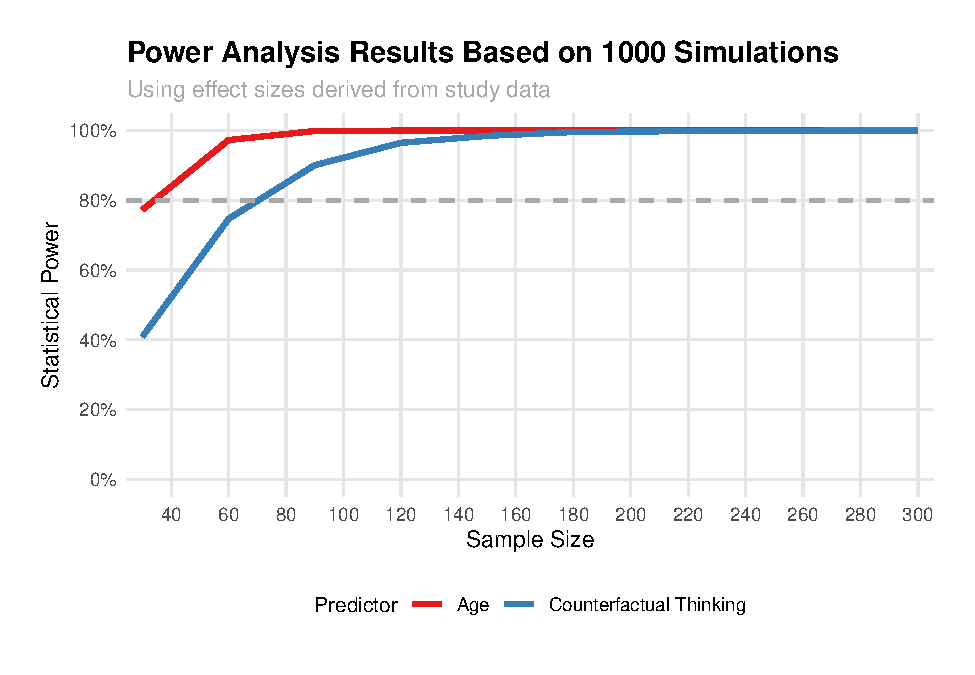
\includegraphics{final_project_files/figure-latex/unnamed-chunk-9-1.pdf}

\begin{Shaded}
\begin{Highlighting}[]
\CommentTok{\# Calculate required sample sizes for 0.8 power}
\NormalTok{age\_n }\OtherTok{\textless{}{-}} \FunctionTok{min}\NormalTok{(power\_results}\SpecialCharTok{$}\NormalTok{n[power\_results}\SpecialCharTok{$}\NormalTok{power\_age }\SpecialCharTok{\textgreater{}=} \FloatTok{0.8}\NormalTok{])}
\NormalTok{cf\_n }\OtherTok{\textless{}{-}} \FunctionTok{min}\NormalTok{(power\_results}\SpecialCharTok{$}\NormalTok{n[power\_results}\SpecialCharTok{$}\NormalTok{power\_cf }\SpecialCharTok{\textgreater{}=} \FloatTok{0.8}\NormalTok{])}

\FunctionTok{cat}\NormalTok{(}\StringTok{"Required sample sizes for 80\% power:}\SpecialCharTok{\textbackslash{}n}\StringTok{"}\NormalTok{,}
    \StringTok{"Age effect:"}\NormalTok{, age\_n, }\StringTok{"participants}\SpecialCharTok{\textbackslash{}n}\StringTok{"}\NormalTok{,}
    \StringTok{"Counterfactual thinking effect:"}\NormalTok{, cf\_n, }\StringTok{"participants}\SpecialCharTok{\textbackslash{}n}\StringTok{"}\NormalTok{)}
\end{Highlighting}
\end{Shaded}

While our analysis revealed significant effects with this sample size, the power analysis suggests that future research would benefit from larger samples to detect the relationship between counterfactual thinking and conservation abilities more reliably. This disparity between our actual sample size and the recommended sample size from the power analysis doesn't invalidate our findings, but rather contextualizes them and provides valuable guidance for future research. The significant effects found with our relatively modest sample size might actually suggest that the relationship between counterfactual thinking and conservation abilities is stronger than initially hypothesized, as these effects were detectable even under conditions of lower statistical power. Nevertheless, future studies should aim to achieve higher statistical power.

To achieve better power, several strategies could be considered. First, increasing the number of trials per participant would enhance the sensitivity of the counterfactual thinking measures. Additionally, controlling for known sources of variance in children's performance, such as language ability and working memory capacity (executive function), could improve the signal-to-noise ratio. These adjustments would strengthen the statistical power detect true effects without necessarily requiring a substantially larger sample size, though increasing the sample size remains a viable option if resources allow.


\end{document}
